\documentclass[letterpaper]{article}

\usepackage{fixltx2e}
\usepackage{algorithm2e}
\usepackage{graphicx}
\usepackage{amsmath}
\usepackage{cite}
\usepackage{amssymb}
\usepackage{mathrsfs}
\usepackage{gensymb}
\usepackage{aaai} 
\usepackage{times} 
\usepackage{helvet} 
\usepackage{courier} 
\setlength{\pdfpagewidth}{8.5in} 
\setlength{\pdfpageheight}{11in} %%%%%%%%%%
% PDFINFO for PDFLATEX
% Uncomment and complete the following for metadata (your paper must compile with PDFLATEX)
\pdfinfo{
}%%%%%%%%%%
% Section Numbers
% Uncomment if you want to use section numbers % and change the 0 to a 1 or 2
% \setcounter{secnumdepth}{0} %%%%%%%%%%
% Title, Author, and Address Information 

%\title{Climate control for performant HPUs}
\title{Hysteresis effects in image labelling}
\author{Authors undisclosed}

%%%%%%%%%%
% Body of Paper Begins
\begin{document}
\maketitle

%\usepackage{multirow}


\begin{abstract}
	It is well known in psychology that priming can bias people toward giving
	certain responses in a task.  We investigate to what extent this mechanism 
	comes into play for workers performing image-labelling tasks on the
	microtask platform Amazon Mechanical Turk.  
	We first present an algorithmic definition of priming, and then apply this
	definition to show that workers become primed simply by the previous 
	tasks they have performed, in the sense that a classifier can reliably
	infer the treatment from which a worker was drawn.
	In an image labelling task, varying the images presented in earlier tasks, 
	influences workers focus and specificity
	and demonstrates that a combination of positive priming, negative priming,
	and novelty contribute to the effects observed.
	To obtain greater detail-orientation in the image labelling task, 
	workers should be presented with
	tasks that are as similar to one another as possible.
\end{abstract}
\textbf{}
\section*{Introduction}

Although capabilities in artificial intelligence continue to advance, 
there are still many tasks for which human performance exceeds that of 
computers now and in the forseeable future.  Tasks requiring repertoire of 
general knowledge about the world, the use of common sense or expert judgment, 
finding creative solutions to open-ended questions, and spontaneously 
hypothesis generation outside any apparent framework, are all examples of 
tasks that are routine for humans, but very difficult or impossible for 
computers.  The image labelling task is perhaps the canonical human 
intelligence task (HIT), perhaps because it is simply stated, nearly effortless
for humans, but still extremely challenging for computers.

Rather than replicate human intelligence, there is an alternate vision in 
which human intelligence can be freely accessed and meshed with artificial
intelligenc.  The emergence of microtask platforms like Amazon Mechanical 
Turk (AMT) has made this vision a reality to some extent.  In this paradigm,
the human processing unit (HPU) becomes one component in a hybrid 
computational system, analogous to the CPU \cite{5543192}.

But there are major challenges in building systems that deliver on this 
vision\cite{kittur2008crowdsourcing}.  People are far more complex than manufactured chips, 
and so HPU performance is noisy, and subject to bias, leading to uncertain
quality of output.  Of course, the effect that HPU noise has on a compute job 
will depend on the application.
In the image labelling task, some variability is desirable, because it helps
generate sets of labels that in some sense cover semantic space occupied by an 
image.  In other cases this variability can be problematic.  In a 
transcription task, usually there is only one correct output, and so 
variability in the output only degrades quality.

Regardless of the application, the understanding HPU variance quantitatively,
and the factors that influence it, will help design of efficient compute 
systems built from HPUs.

Much has been written on the factors that influence human input in 
crowdsourcing platforms.  This has generally related to the context in which
the HPU engages the task.  Unfortunately, especially for platforms like AMT,
this context is out of the designers control, and the relative anonymity of
workers makes it difficult to select for specific conditions.

In the present work, we compare influences that arise from the framing of the
task to influences that arise in-task from the mere act of working.  What 
are the effects of performance that arise simply from how the worker's 
attention is influenced by the previous task, and how do these relate 
quantitatively to other pre-task influences?

We pay workers on AMT to label images, and analyze the effects brought about
by subjecting them to different priming treatments, either in the form of 
disclosing a semantically charged name of a (fictitious) organization 
funding the research, or by altering the first few images presented to the
workers.  Surprisingly, simply altering the first few images produces a much
stronger shift in subsequent labelling performance than does disclosing the 
semantically-laden name of the funder. 



\section*{Prior Work}


When considering the design of computing systems based on HPUs, we can think
of variability in HPU output as having a relatively persistent component,
and a transient one.  The persistent component would include intrinsic
qualities of a person, such as their temperament, life history, and their 
current developmental stage.  Such characteristics cannot be influenced by
the designer, but it may be possible to screen or at least characterize them 
to some extent.

The transient component of variability might include such factors as influence
alertness, orientation focus, mood, meaningfulness of the task, and any number
of aspects of mental state too subtle to describe.  Such aspects are partly
in the control of the system designer, and can be controlled through how the
task is framed and set up.

In psychology, the phenomenon of priming occurs when a prior stimulus 
makes a person more likely to respond to a task in a particular way
\cite{schvaneveldt1973retrieval, No2007}.  The 
phenomenon is well-studied, and is believed to follow perceptual, semantic,
or conceptual similarities between the priming stimulus and the ensuing 
response.

Drawing from this insight, it is natural to wonder whether current HPU 
performance might be modulated by recently performed tasks.

Existing work on the effects of human input in crowdsourcing platforms has
generally focused on effects arising from auxiliary information, which has
been added into the task setting, or which frames the task during its 
introduction.  

For example, it was shown that framing a task in a meaningful or meaningless
way influences both task quality and the willingness of workers to produce
more output given a declining payment schedule.
Surprisingly, relative to a zero-context treatment, although workers who were
told that there contributions would be used to help identify cancerous cells
were willing to provide more work, their work was not of a sufficiently higher
quality.  The only effect on quality occered when workers were told that their
output would be discarded, in which case quality declined.

Another study investigated the influence of providing workers with information
about one another.  This study found that workers were willing to provide
more output, when they were able to see one another's names.  The effect was 
stronger when workers could also see some basic self-reported demographic 
information, and more still when they could see one another's responses.

In the present work, we focus on a perhaps unusual source of priming---that 
arising from the task itself, and compare this to priming that results from 
framing the work as part of study by a named organization.  Given that the 
mechanisms of priming are believed to be related to the residual activation of
perceptual, semantic, and conceptual representations, we hypothesize that 
\textit{in-task} priming could produce effects quantatively comparable to those
produced by framing.

\section*{Theoretical Framework}
Having discussed very briefly some mechanisms and cases of priming, we shall 
now seek to put forward, as an additional testable contribution, a rigorous
definition for priming that is suitable for the study of computing with HPUs.

First, we remark that it does not make sense to speak of an un-primed 
state.  When a person engages in a task, she comes to the task with some 
state of mind.  We therefore do not attempt to define priming in an absolute
sense, but rather, in a relative sense, that is, one priming can be said to 
be different from another.

Also, the effects of a given treatment will depend on the task to which the 
HPUs are put.  In other words, a treatment which generates a strong effect on
the output in one task, does not necessarily produce a strong effect on the
output for other tasks.  On a related note, the study of the effects of priming
on HPUs should be defined algorithmically.  Only effects on HPU output that
can be detected algorithmically can be relevant to a computing system built 
from HPUs.

Further, since only the influence on populations of HPU outputs can be 
meaningfully measured, and since accessing HPU power generally involves 
sampling from a pool of HPU workers, we define priming as a property of a 
population of HPU outputs.  Having said these remarks, we now present an
algorithmic definition of HPU priming:

Two populations of HPU outputs, \textsc{j} and \textsc{k}, are said to be 
\textit{differently primed} with respect to a task $\mathcal{T}$ if there 
exists an algorithm $\mathcal{A}$ which runs in time polynomial in the size
of \textsc{j} and \textsc{k}, that can distinguish 
(classify) members of \textsc{j} and \textsc{k} with accuracy 
$\frac{1+\theta}{2}$, on input \textsc{j} and \textsc{k}.  Further, $\theta$
must be a non-negligible function of $|\textsc{j} + \textsc{k}|$.
If such an $\mathcal{A}$ exists, 
we say that \textsc{j} and \textsc{k} deviate by $\theta$ in priming.

The above definition is simply intended to provide a well-defined definition
of what priming \textit{is}.  Naturally, it says nothing about the consequences
of priming.  The significance of the priming of a given population will
depend both on the nature of $\mathcal{T}$ and on the intended purpose of 
the work products derived from HPUs performing $\mathcal{T}$.


\section*{Methods}

\textbf{Task set-up.}
We paid 900 AMT workers to perform an image-labelling task.  A task consisted 
of labelling 10 images, with 5 labels each.  The first 5 images were varied 
depending on the priming treatment, while the last 5 images were the same 
across all treatments.  Ordering of the images was kept constant.

Workers were randomly assigned to one of 6 treatments.  The treatments differed
from one another along two dimensions. The first dimension consisted of 
varying the first 5 images shown to the worker.  This was used to test the
effects of \textit{in-task} priming.

The second dimension concerned disclosure of a (fictitious) organization,
purportedly funding work as part of a research study.  Depending on the 
treatment, one of two funding agencies was presented, or no indication was 
made.

Tasks were presented to workers as a series of panels or flash cards.  The
first panel provided brief instructions, and was identical for all treatments.
Workers could see this panel when previewing the task, but could not advance.
Depending on the treatment, the worker was either shown a second panel 
stating the name of 
one of two fictitious organizations funding the work, or this panel was 
skipped.  The next five panels each consisting of a priming sub-tasks, 
wherein the worker was asked to submit five descriptive labels.  The images
used during the priming sub-task depended on the treatment.  The last 5 panels
consisted of testing subtasks, wherein, as for the priming sub-tasks, workers
were asked to submit 5 descriptive labels.

\begin{table*}[t]
\centering
	\begin{tabular}{ l  c  l }
		\hline                       
		Treatment & Funder & Image Set	\\ 
		\hline                       
		$\textsc{ambg}$ & None & Ambiguous meals\\
		$\textsc{cult}_{img}$ & None & Cultural meals\\
		$\textsc{cult}_{fund}$ & The Global Foundation for Cultural Recognition& Cultural meals\\
		$\textsc{cult}_{fund,img}$ & The Global Foundation for Cultural Recognition& Cultural meals\\
		$\textsc{ingr}_{img}$ & None & Separated ingredients\\
		$\textsc{ingr}_{fund}$ & The National Foundation for Nutritional Awareness & Separated ingredients\\
		$\textsc{ingr}_{fund, img}$ & The National Foundation for Nutritional Awareness   & Separated ingredients\\
		\hline  
	\end{tabular}
	\caption{Treatments to which Amazon Mechanical Turk workers were 
		placed when asked to perform an image labelling task. The images
		used in the image sets are reproduced in 
		Figs.~\ref{fig:testImages}, \ref{fig:ambiguous}, \ref{fig:cultural}, and \ref{fig:ingredients}.
	}
	\label{table:1}
\end{table*}

%\begin{tabular*}{ l  c  r }
%	\hline                       
%	Treatment & Funder & Image Set	\\ 
%	\hline                       
%	$\textsc{ambg}$ & None & Cultural\\
%	$\textsc{cult}_{img}$ & None & Cultural\\
%	$\textsc{cult}_{fund}$ & \begin{tabular}[x]{@{}c@{}}The Global Foundation\\for Cultural Recognition\end{tabular}    & Cultural\\
%	$\textsc{cult}_{fund,img}$ & \begin{tabular}[x]{@{}c@{}}The Global Foundation\\for Cultural Recognition\end{tabular}    & Cultural\\
%	$\textsc{ingr}_{img}$ & None & Cultural\\
%	$\textsc{ingr}_{fund}$ & \begin{tabular}[x]{@{}c@{}} The National Foundation\\ for Nutritional Awareness\end{tabular}      & Cultural\\
%	$\textsc{ingr}_{fund, img}$ & \begin{tabular}[x]{@{}c@{}} The National Foundation\\ for Nutritional Awareness\end{tabular}  & Cultural\\
%	\hline  
%\end{tabular*}

\textbf{Choice of images.}
The 5 test images, were chosen with two ideals in mind.  
First, we chose images that we judged would generate a diverse vocabulary of 
labels, such that the effects of priming could be detected.  In other words,
sparse images with a single object in the foreground were not considered good 
candidates, since they would be less likely to elicit labels that varied from 
one worker and one priming treatment to the next.

Second, we chose images which would produce labels belonging to two broad
concepts, which would serve as the targets of our priming: food and culture.  
This created the opportunity to attempt to prime workers in a way that would
bias them toward emitting food-related or culture-related labels.

Under these considerations, we chose the images shown in 
Fig.~\ref{fig:testImages}.  Each of these images has food as its main focus,
but also has a strong and specific cultural reference due to the unique, 
iconic character of the food and the artifacts depicted.

To investigate in-task priming, we chose a set of images that highly
recognizable cultural settings and no food, and another set that contained
separated food ingredients, without any overt cultural content.  The third
set of images was chosen to be very much like the test images, showing prepared
meals, and though prepared food is inseparable from culture, these images
were chosen based on being culturally more muted or ambiguous. 

\textbf{Label ontology.}
In order to provide a deeper analysis, we built an ontology
of the corpus of all labels applied to the first test image.  The ontology
was built as a directed acyclic graph starting 

We next look at how alternately treated HPUs differ in their tendency to use
more specific or more general labels. We use the ontology of labels emitted
on the first test image to unambiguously establish a partial ordering of 
label-specificity.  If one label $\ell_1$ is within the ancestry of another
$\ell_2$, we say that $\ell_1$ is more general than $\ell_2$, otherwise they
are not comparable.  Thus, the label \texttt{naan} is more 
specific than both \texttt{bread} and \texttt{indian}, while incomparable to
\texttt{statue}.

\section*{Results and discussion}

\begin{figure*}
	\begin{center}
		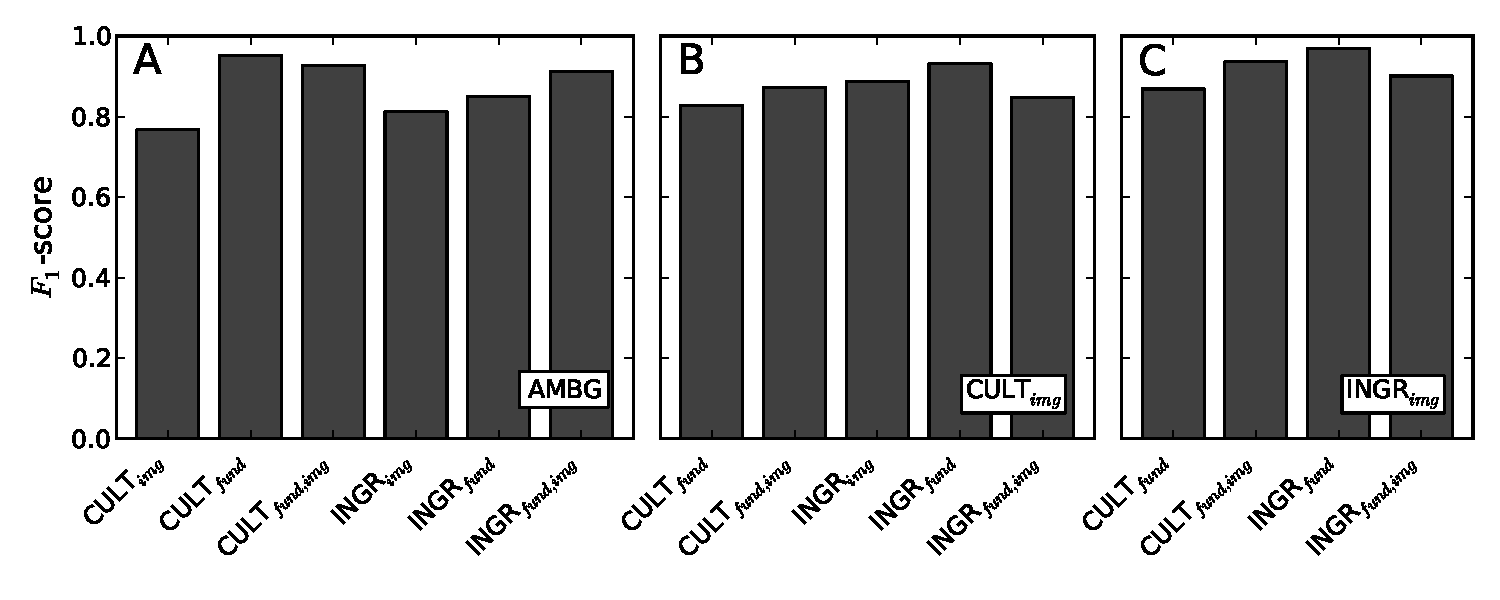
\includegraphics[scale=0.55]{../figs/f1scores.pdf}
		\caption{$F_1$-score for binary classification of HPUs from separate
			treatments using a naive Bayes classifier.  Each panel shows
			the performance of the classifier when distinguishing between 
			a basis treatment (inset) and the treatments listed on the 
			abscissa.
		}
		\label{fig:classifier}
	\end{center}
\end{figure*}

\textbf{Priming affects HPU output.}
We first demonstrate that in a completely general sense, the priming treatments
had a noticeable effect on the labels that workers assigned to images.  We
test this by building a naive Bayes, which distinguishes workers from 
different treatments based on the labels they submitted for the test images.

\begin{figure}
	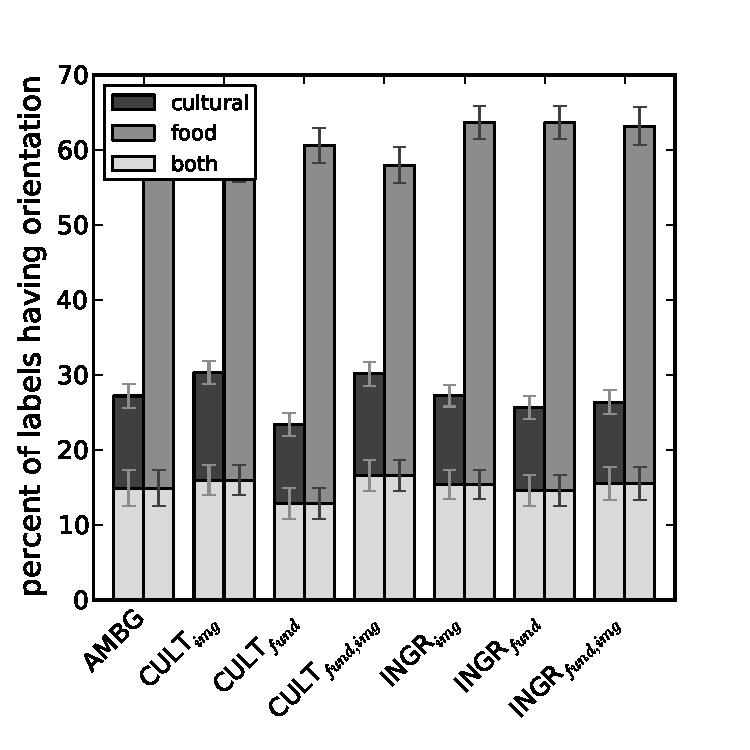
\includegraphics[scale=0.65]{../figs/valenceComparison.pdf}
	\caption{Percentage of labels of a food- or cultural- orientation, or
	both.  In our ontology of labels, a label can have multiple parents. 
	For example \texttt{naan} inherits from both \texttt{food} and 
	\texttt{cultural} through its parent \texttt{indian food}.}
	\label{fig:valence}
\end{figure}

Fig.~\ref{fig:classifier}A shows the F1-score for the binary classification 
of workers from $\textsc{ambg}$ and each of the other treatments.  The 
classifier is able to distinguish workers from these treatments with high
sensitivity and precision.  This clearly demonstrates that these treatments
are \textit{differently primed}.  In panel B of Fig.~\ref{fig:classifier}, 
we show $F_1$-scores achieved for classifications involving $\textsc{cult}_{img}$ the other treatments, while panel C shows scores for classifications 
involving $\textsc{ingr}_{img}$ and the other treatments.  In each case, 
the naive Bayes classifier is capable of efficiently distinguishing the
workers from each pairing of treatments, demonstrating that priming was effective.

While it is not so surprising to find that $\textsc{cult}_x$ treatments are 
can be distinguished from $\textsc{ingr}_x$, it is somewhat remarkable that
$\textsc{cult}_{img}$ and $\textsc{cult}_{fund, img}$ can be distinguished.
Workers from these treatments were both primed in a way to activate cultural concepts, and 
both labelled the same priming pictures.  The same can be said for the 
treatments $\textsc{ingr}_{img}$ and $\textsc{ingr}_{fund, img}$.


\textbf{Priming orients HPU focus.}
The main effect that we expect is that workers primed to focus on culture
would provide more culturally-oriented labels, while workers primed to focus
on ingredients would focus more on food, in particular focussing in on 
ingredients.  Figure~\ref{fig:valence} presents the fraction of words having
cultural- or food-orientation from each treatment.

The effect of the cultural images, which comprised the first five images shown
to workers from $\textsc{cult}_{img}$ and $\textsc{cult}_{fund, img}$ are
sharply visible.  Not only do they use more culturally-oriented words, more
of these words are exclusively culturally oriented (i.e not being also 
food-oriented). 

Interestingly, we do not observe this effect for $\textsc{cult}_{fund}$.
In-task exposure clearly outweighs the effects introduced by
disclosing the funder of the research.  It is consistent with our view of 
priming as a hysteresis effect. 

Experiments in psychology show that priming is stronger when the modality of
the priming stimulus is the same as that of the target response.  These
results are is consistent with that view.  This suggests that more attention
toward the progression of tasks is due, rather than considering only worker
orientation (training) and the content of individual tasks.

Looking at the orientation of words for the $\textsc{ing}_{x}$ treatments, 
we do not see a significant enrichment in food-related words.
Based on the composition of labels coming from people in the \textsc{ambg} 
treatment, it would seem to be the case that our testing images simply elicit
more food-oriented words in general.  It seems likely that priming in the
toward a concept that is already prominent in the images would 
have a less observable effect overall.


\begin{figure*}
	\begin{center}
	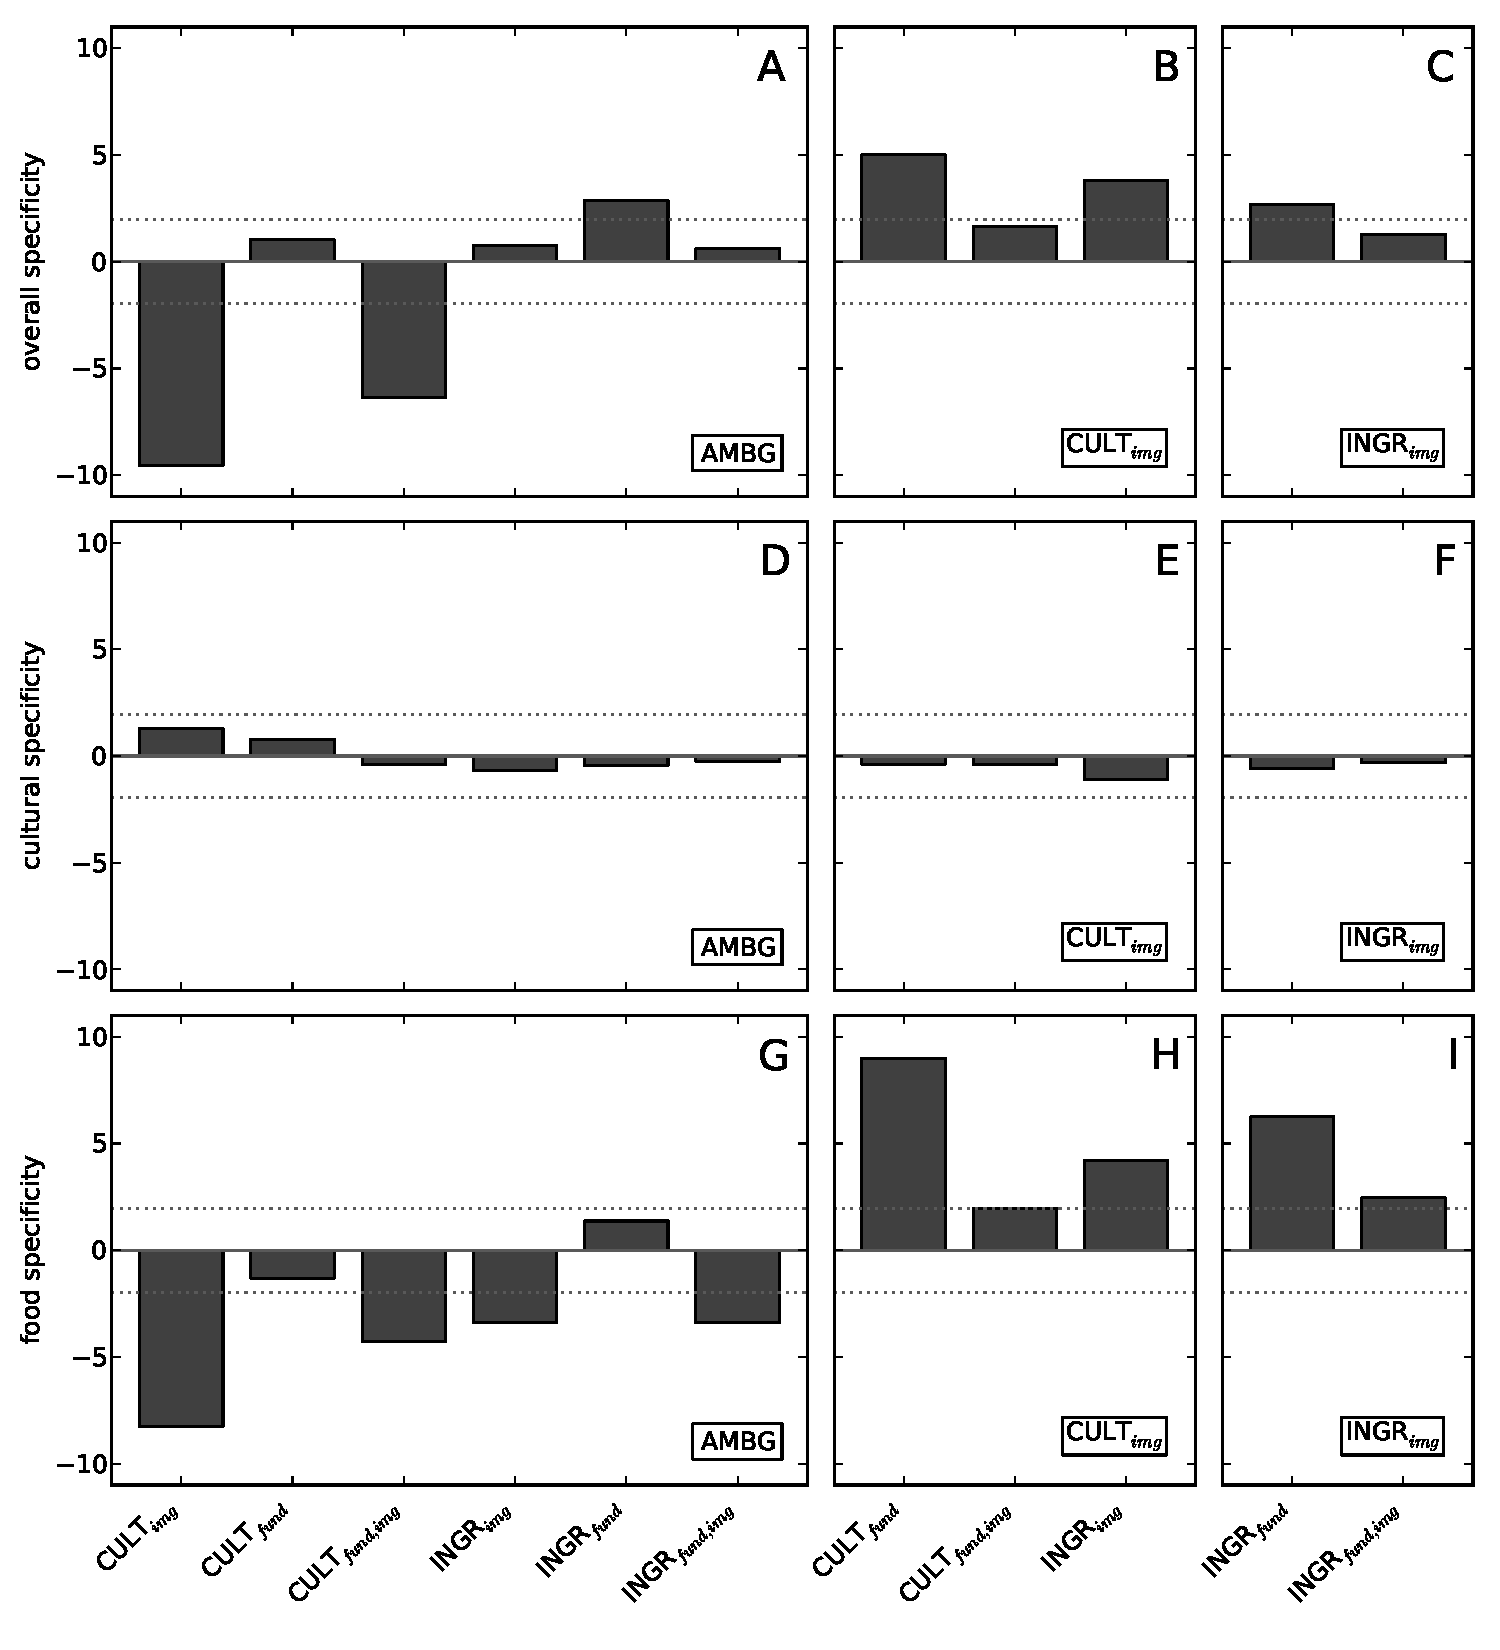
\includegraphics[scale=0.55]{../figs/specificity2.pdf}
	\caption{Pairwise comparisons of label specificity between different 
	HPU treatments.  Each panel presents a binary comparison between a 
	basis treatment (inset) and the subject treatments indicated on the 
	abscissa.  A positive specificity score indicates that the subject 
	treatment emitted more specific words than the basis treatment overall.
	In a given comparison, a sample of 50 HPUs from the   
	each treatment was randomly sampled, and the specificity of labels from
	the HPUs of opposing treatments were compared.
	To compare two HPUs, each pair of labels from different HPUs are compared.
	and the specificity score of subject HPU is the number of cases where its
	label is more specific than the subject HPUs, less the number of cases 
	where it is more general. This score is 
	averaged for all HPU pairings.  Statistical significance is gauged
	by generating a null-comparison between two mutually exclusive subsamples 
	from the basis treatment.  This null-comparison yields a distribution
	of relative specificities whose mean is in principle zero.  The 
	specificity scores are expressed in terms of standard deviations of
	the null-comparison specificities.  
	The dotted lines represent the 95\% confidence interval for rejecting 
	the null Hypothesis that the basis treatment and subject treatment are
	equally specific.
	}
	\label{fig:specificity}
	\end{center}
\end{figure*}

\textbf{Priming affects attention to detail.}
We next investigate whether our priming conditions differ in the degree of 
generality of the labels they submit.  For instance, it is natural to expect
that in the the exposure to isolated ingredients and emphasis on nutrition
in the $\textsc{ingr}_x$ conditions would predispose workers to provide 
labels that name specific ingredients.

Using the ontology generated from the labels of testing image 1 
(Fig.~\ref{fig:testImages}.1), we are able to compare each treatment in respect
of the specificity of words used.  
In Fig.~\ref{fig:specificity}, We show relative specificity scores in 
pairwise comparisons between treatments. Because an ontology only induces a 
partial ordering, it is only possible to perform binary comparisons between
between treatments.

Figure~\ref{fig:specificity}A compares \textsc{ambg} with all other 
treatments.  Both treatments
primed with cultural images ($\textsc{cult}_{img}$ and 
$\textsc{cult}_{fund, img}$) exhibit more labelling compared
to \textsc{ambg}.  Although, $\textsc{ingr}_{fund}$ emitted an excess of 
more specific words.

To try to see whether certain treatments are more specific within labels of 
a given orientation, we can make specificity comparisons while restricting
to words of a cultural or food orientation.  These comparisons are respectively
shown for comparisons to $\textsc{ambg}$ in
Figs.~\ref{fig:specificity}D and G.  In panel D, we can see that, although
$\textsc{cult}_{img}$, and $\textsc{cult}_{fund, img}$ were enriched in the 
\textit{amount} of cultural words, they do not use more \textit{specific}
cultural words.

One simple explanation for these observations is that  would be that people 
generally have more specific words for food-related concepts than for cultural 
ones.  This would certainly stand to reason, in which case one would expect
to see an enrichment in the quantity of cultural words, while the increase
in specificity might be more difficult to measure.

Explaining the results for $\textsc{ingr}_{x}$ in panel D is more subtle,
however.  As we mentioned above, one would expect that priming for ingredients
and nutrition would elicit more specific words, but this is not observed for
the two treatments in which the first five images featured isolated 
ingredients.  In fact, these treatments showed significantly \textit{less}
specificity.  

This surprising result and, along with the other results in panels A, D, and G
can be explained if we consider the effects of novelty and negative priming.
Although the ingredients images probably do encourage the workers to focus
to some extent on ingredients, when they encounter the test images, they are
presented with the novelty of prepared meals and table settings.  These 
novelties naturally attract attention and become the subject of labels such
as $\texttt{meal}$.  

Negative priming on the other hand inhibits a person from responding to a
stimulus that is repeated and regarded as not salient \cite{versace2001negative}.  
Workers in the
treatments exposed to the ambiguous image set, who have seen five images
of prepared meals, might then be less likely to respond to the first test
image by submitting $\texttt{meal}$ as one of the labels.

\section{Conclusion}

We provided a novel algorithmic definition for the notion of
priming.  This opens up an avenue for rigorously demonstrating the existence 
of priming by using existing algorithmic tools, such as a naive Bayes 
classifier.  In our study we used this definition to test the effectiveness
of our priming treatments.

Our results demonstrate that a strong hysteresis effect can be observed in 
workers performing an image labelling task.  This in-task priming effect 
appears to be much stronger than that introduced by disclosing the funder
of a study, even when the name of the funder caries an implicit semantic
orientation resonant in the task.

The effects of in-task priming have some degree of subtlety.  While workers
can be primed to focus on certain concepts simply by showing them exemplars, 
the activation of target concepts can be counterbalanced by the novelty of
their absence in subsequent tasks.

It appears to be the case that one can encourage greater specificity in the
labelling task by presenting a series of images that are similar to one 
another.  This suggests a method for obtaining highly specific
labels, by repeatedly putting images out to be labelled, clustering them based
on the labels they recieve, and then re-serving the clustered images to 
workers.  The clustered images will be similar in their gross features, driving
workers to focus on their minutia.

In summary, the hysteresis effect is strong in image labelling tasks, and 
the designer of microtasks would be well-served by considering 
not just the design of individual tasks, but also their progression.


\begin{figure}
	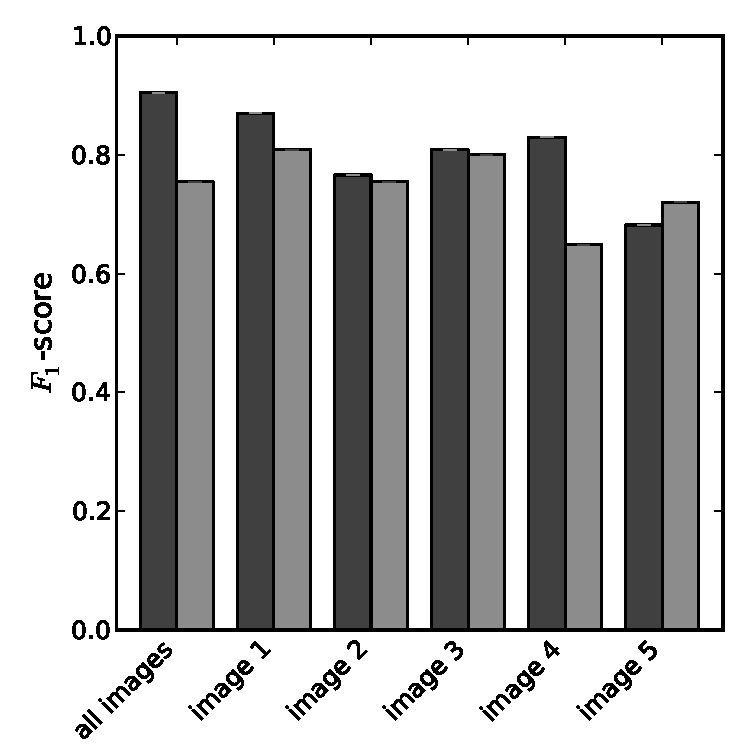
\includegraphics[scale=0.58]{../figs/longitudinalF1scores.pdf}
\caption{$F_1$-score for a naive Bayes classifier trained to distinguish
	HPUs from $\textsc{ingr}_{img}$ and $\textsc{cult}_{img}$ based on 80  
	instances from each treatment, and tested using 20 instances.  Here we
	present the performance of the classifier when only the labels from 
	specific images are presented, to exhibit whether its performance degrades 
	as the number of subtasks since priming increases. 
	}
	\label{fig:longitude}
\end{figure}


One interesting test of this hypothesis arises in 
% Graphics commented out because they make compiling take long!  
% Uncomment when desired!
\begin{figure*}
	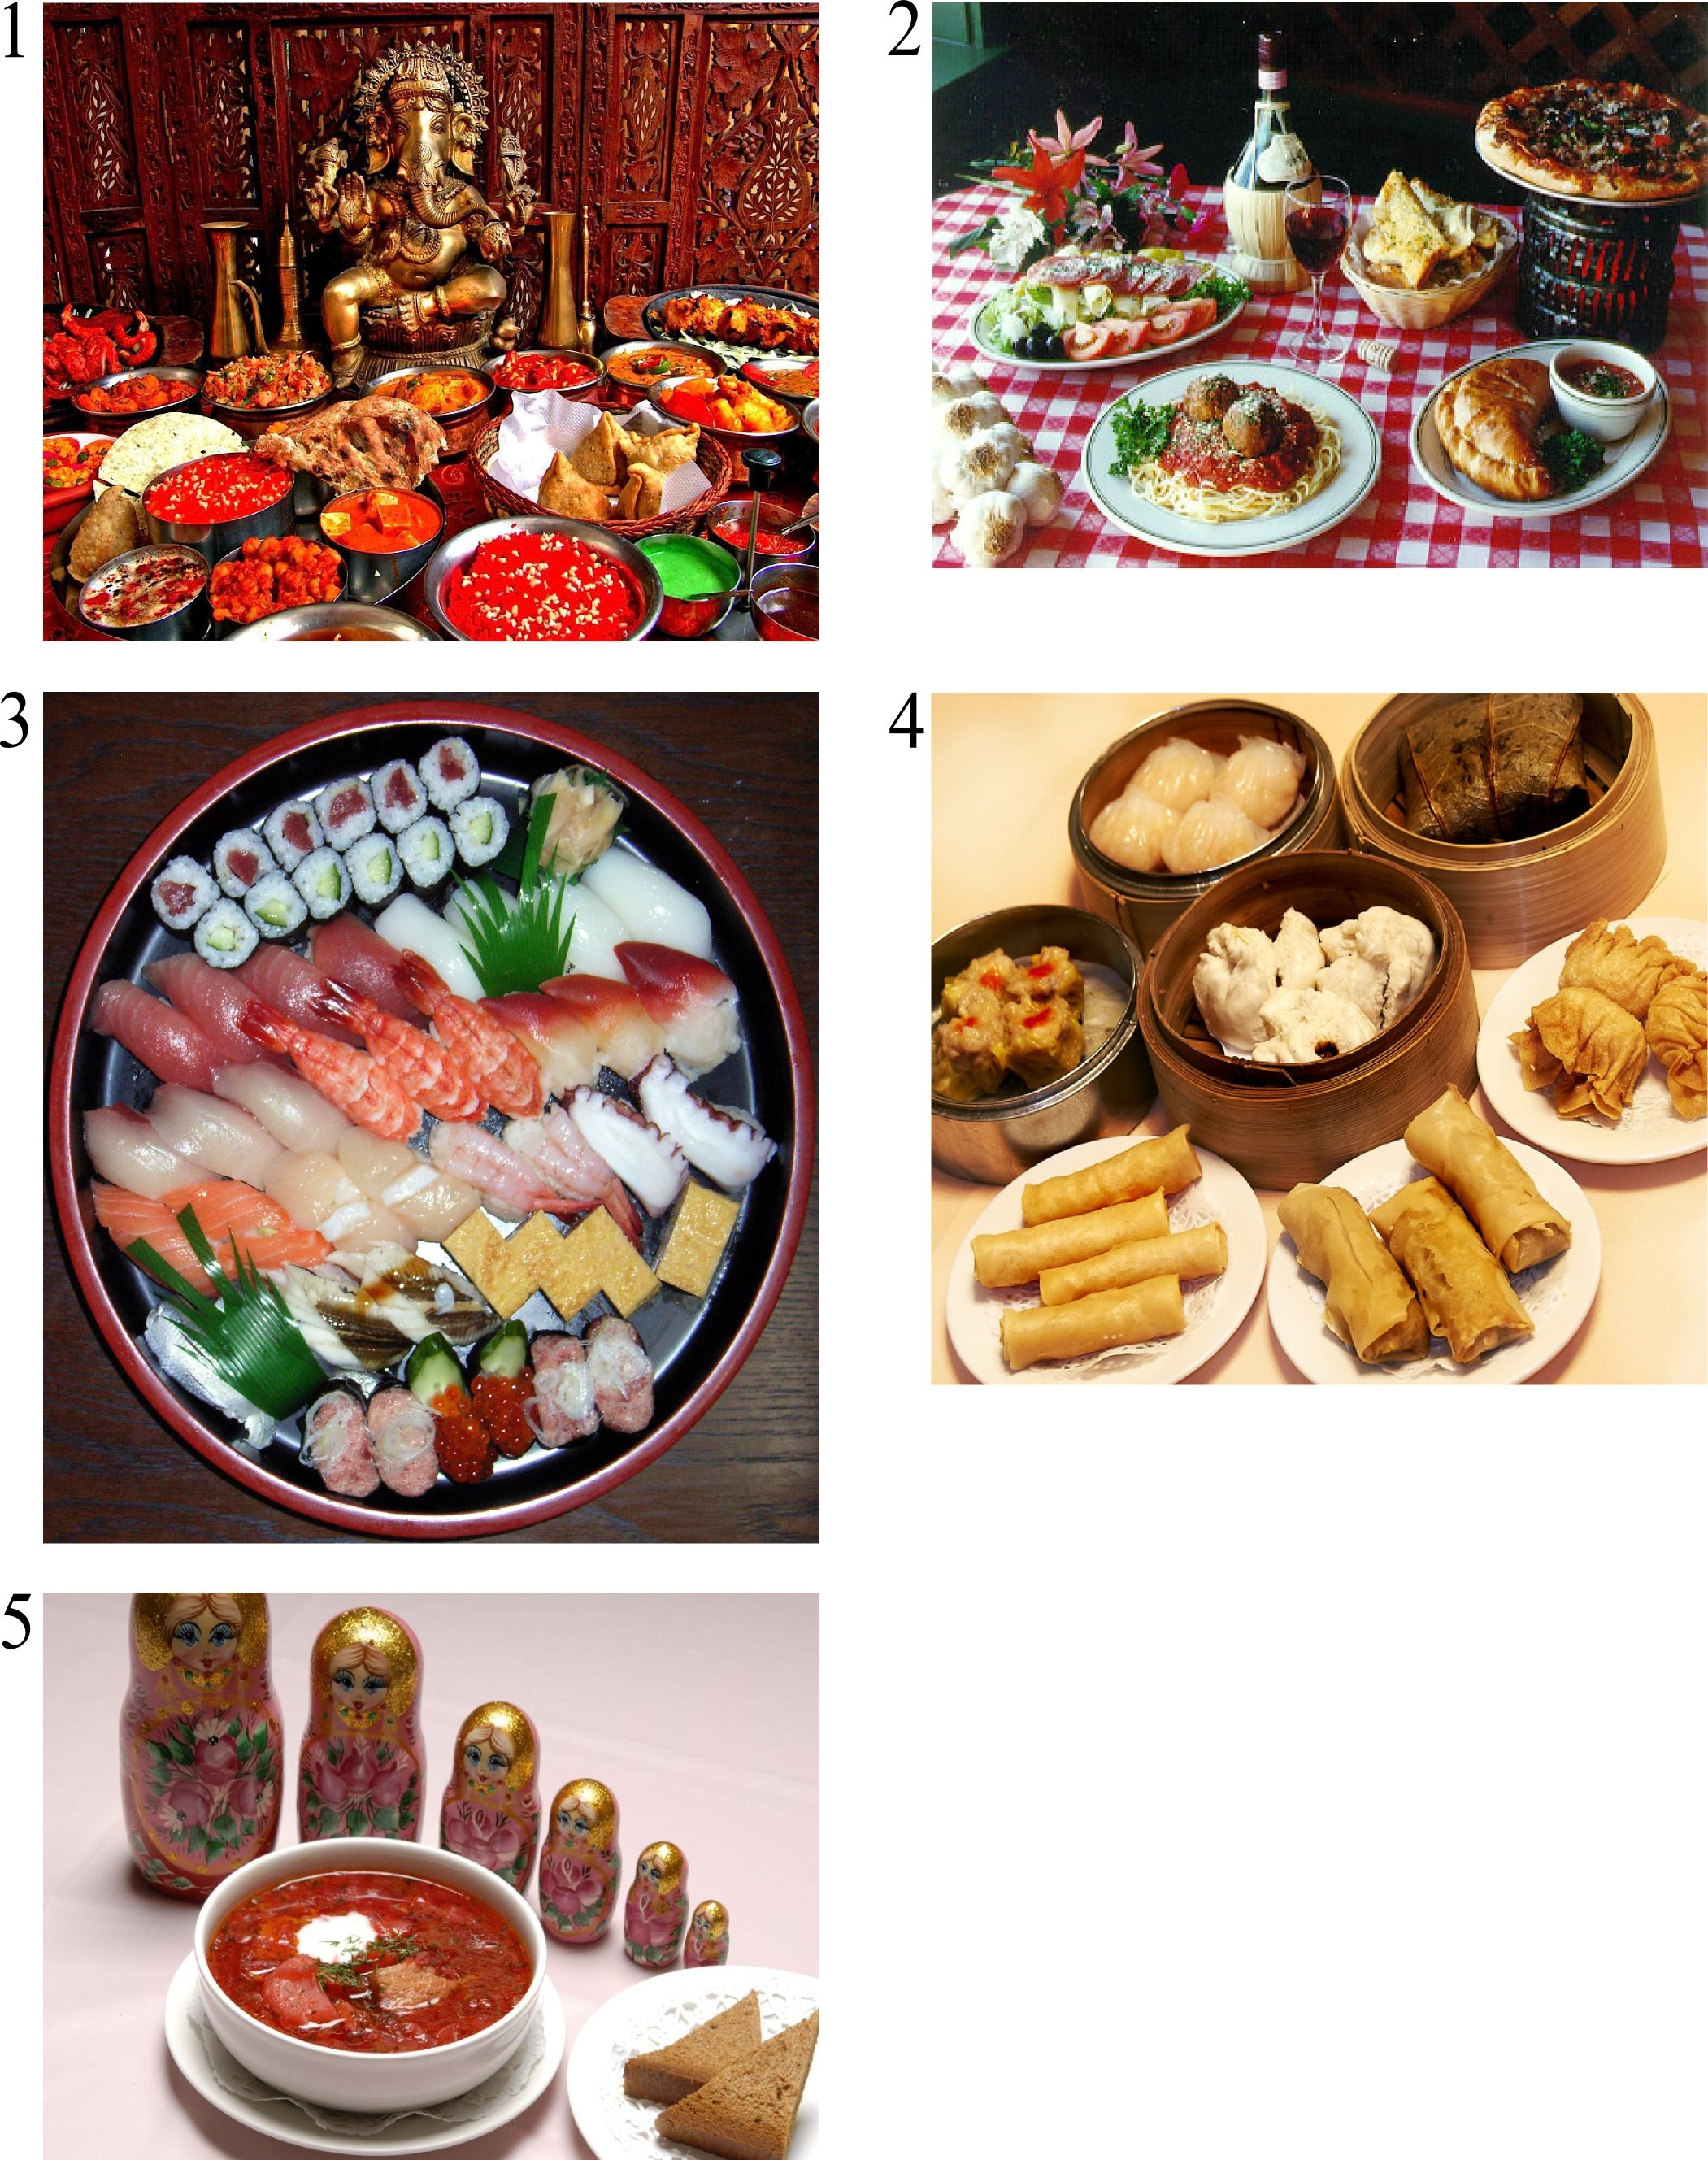
\includegraphics[scale=1.00]{../figs/taskImages/testImages.png}
	\caption{Images used in the testing set.  These images were presented to
	workers after having labelled five other images, either from the cultural
	set (Fig.~\ref{fig:cultural}), ingredients set (Fig.~\ref{fig:ingredients}), or ambiguous set (Fig.~\ref{fig:ingredients}).}
	\label{fig:testImages}
\end{figure*}

\begin{figure*}
	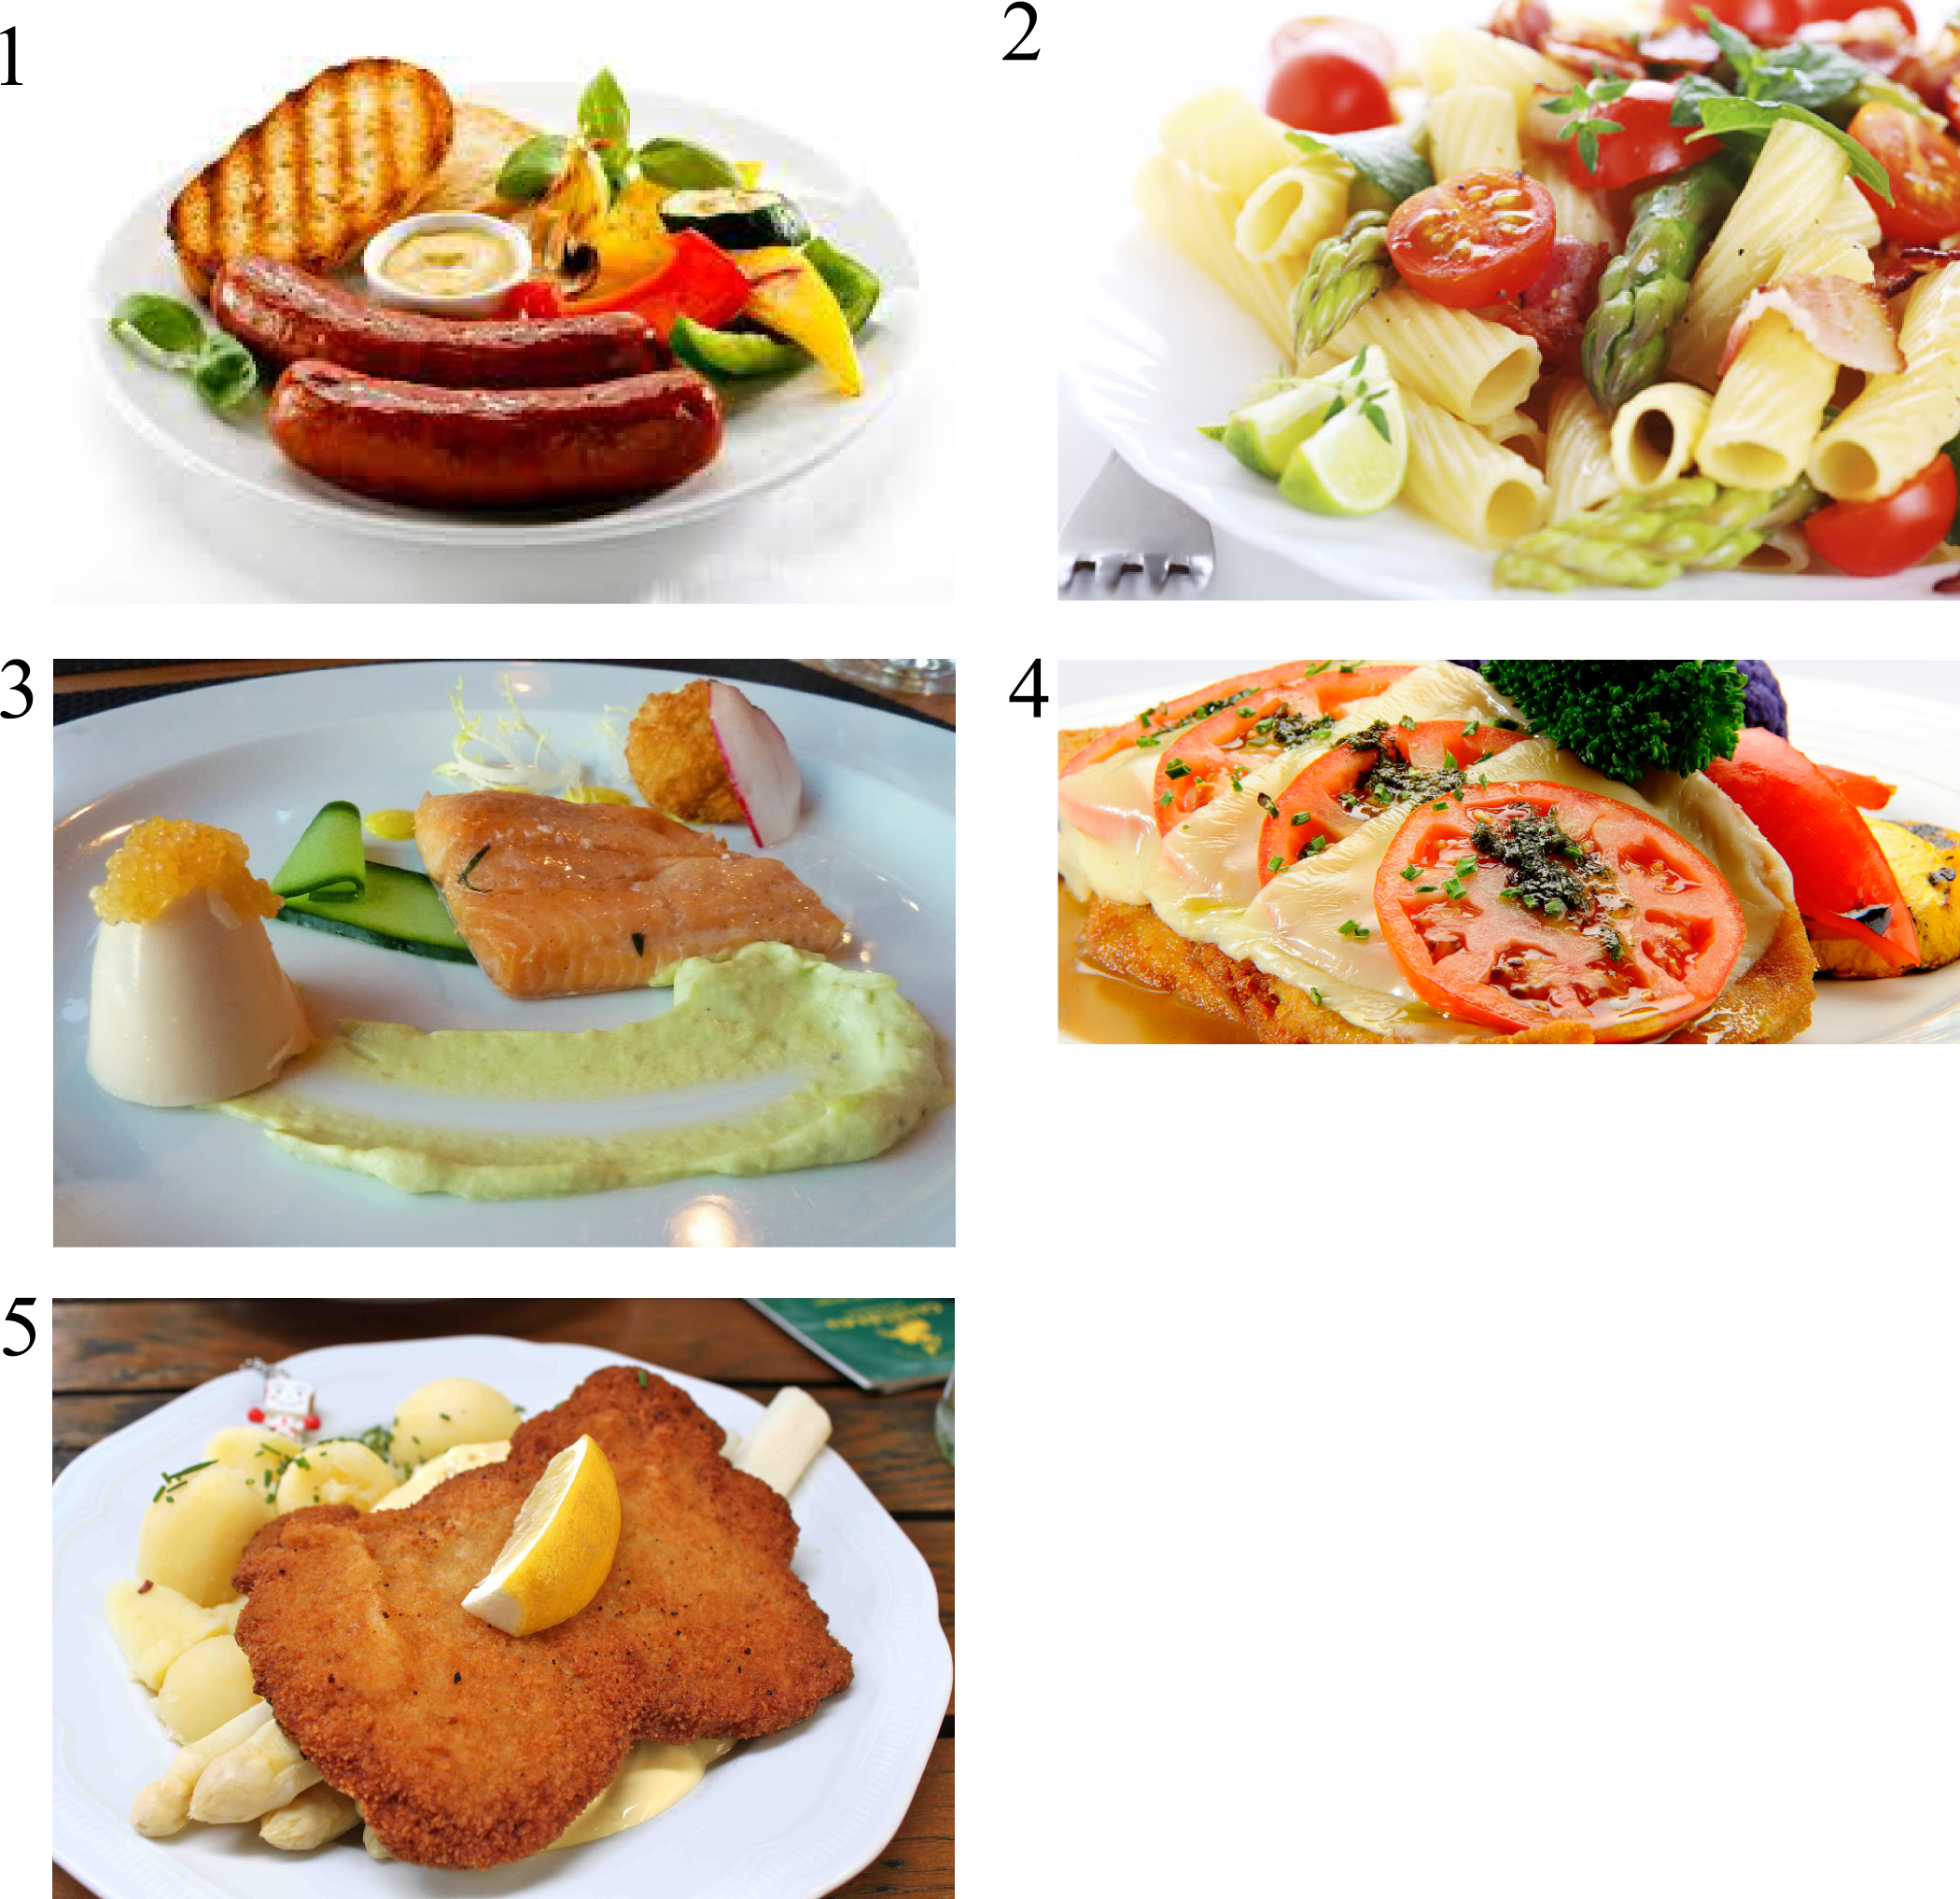
\includegraphics[scale=1.00]{../figs/taskImages/ambiguous.png}
	\caption{Ambiguous image set.  These images were chosen to be similar to 
	the test images, but did not have predominant cultural orientation.}
	\label{fig:ambiguous}
\end{figure*}

\begin{figure*}
	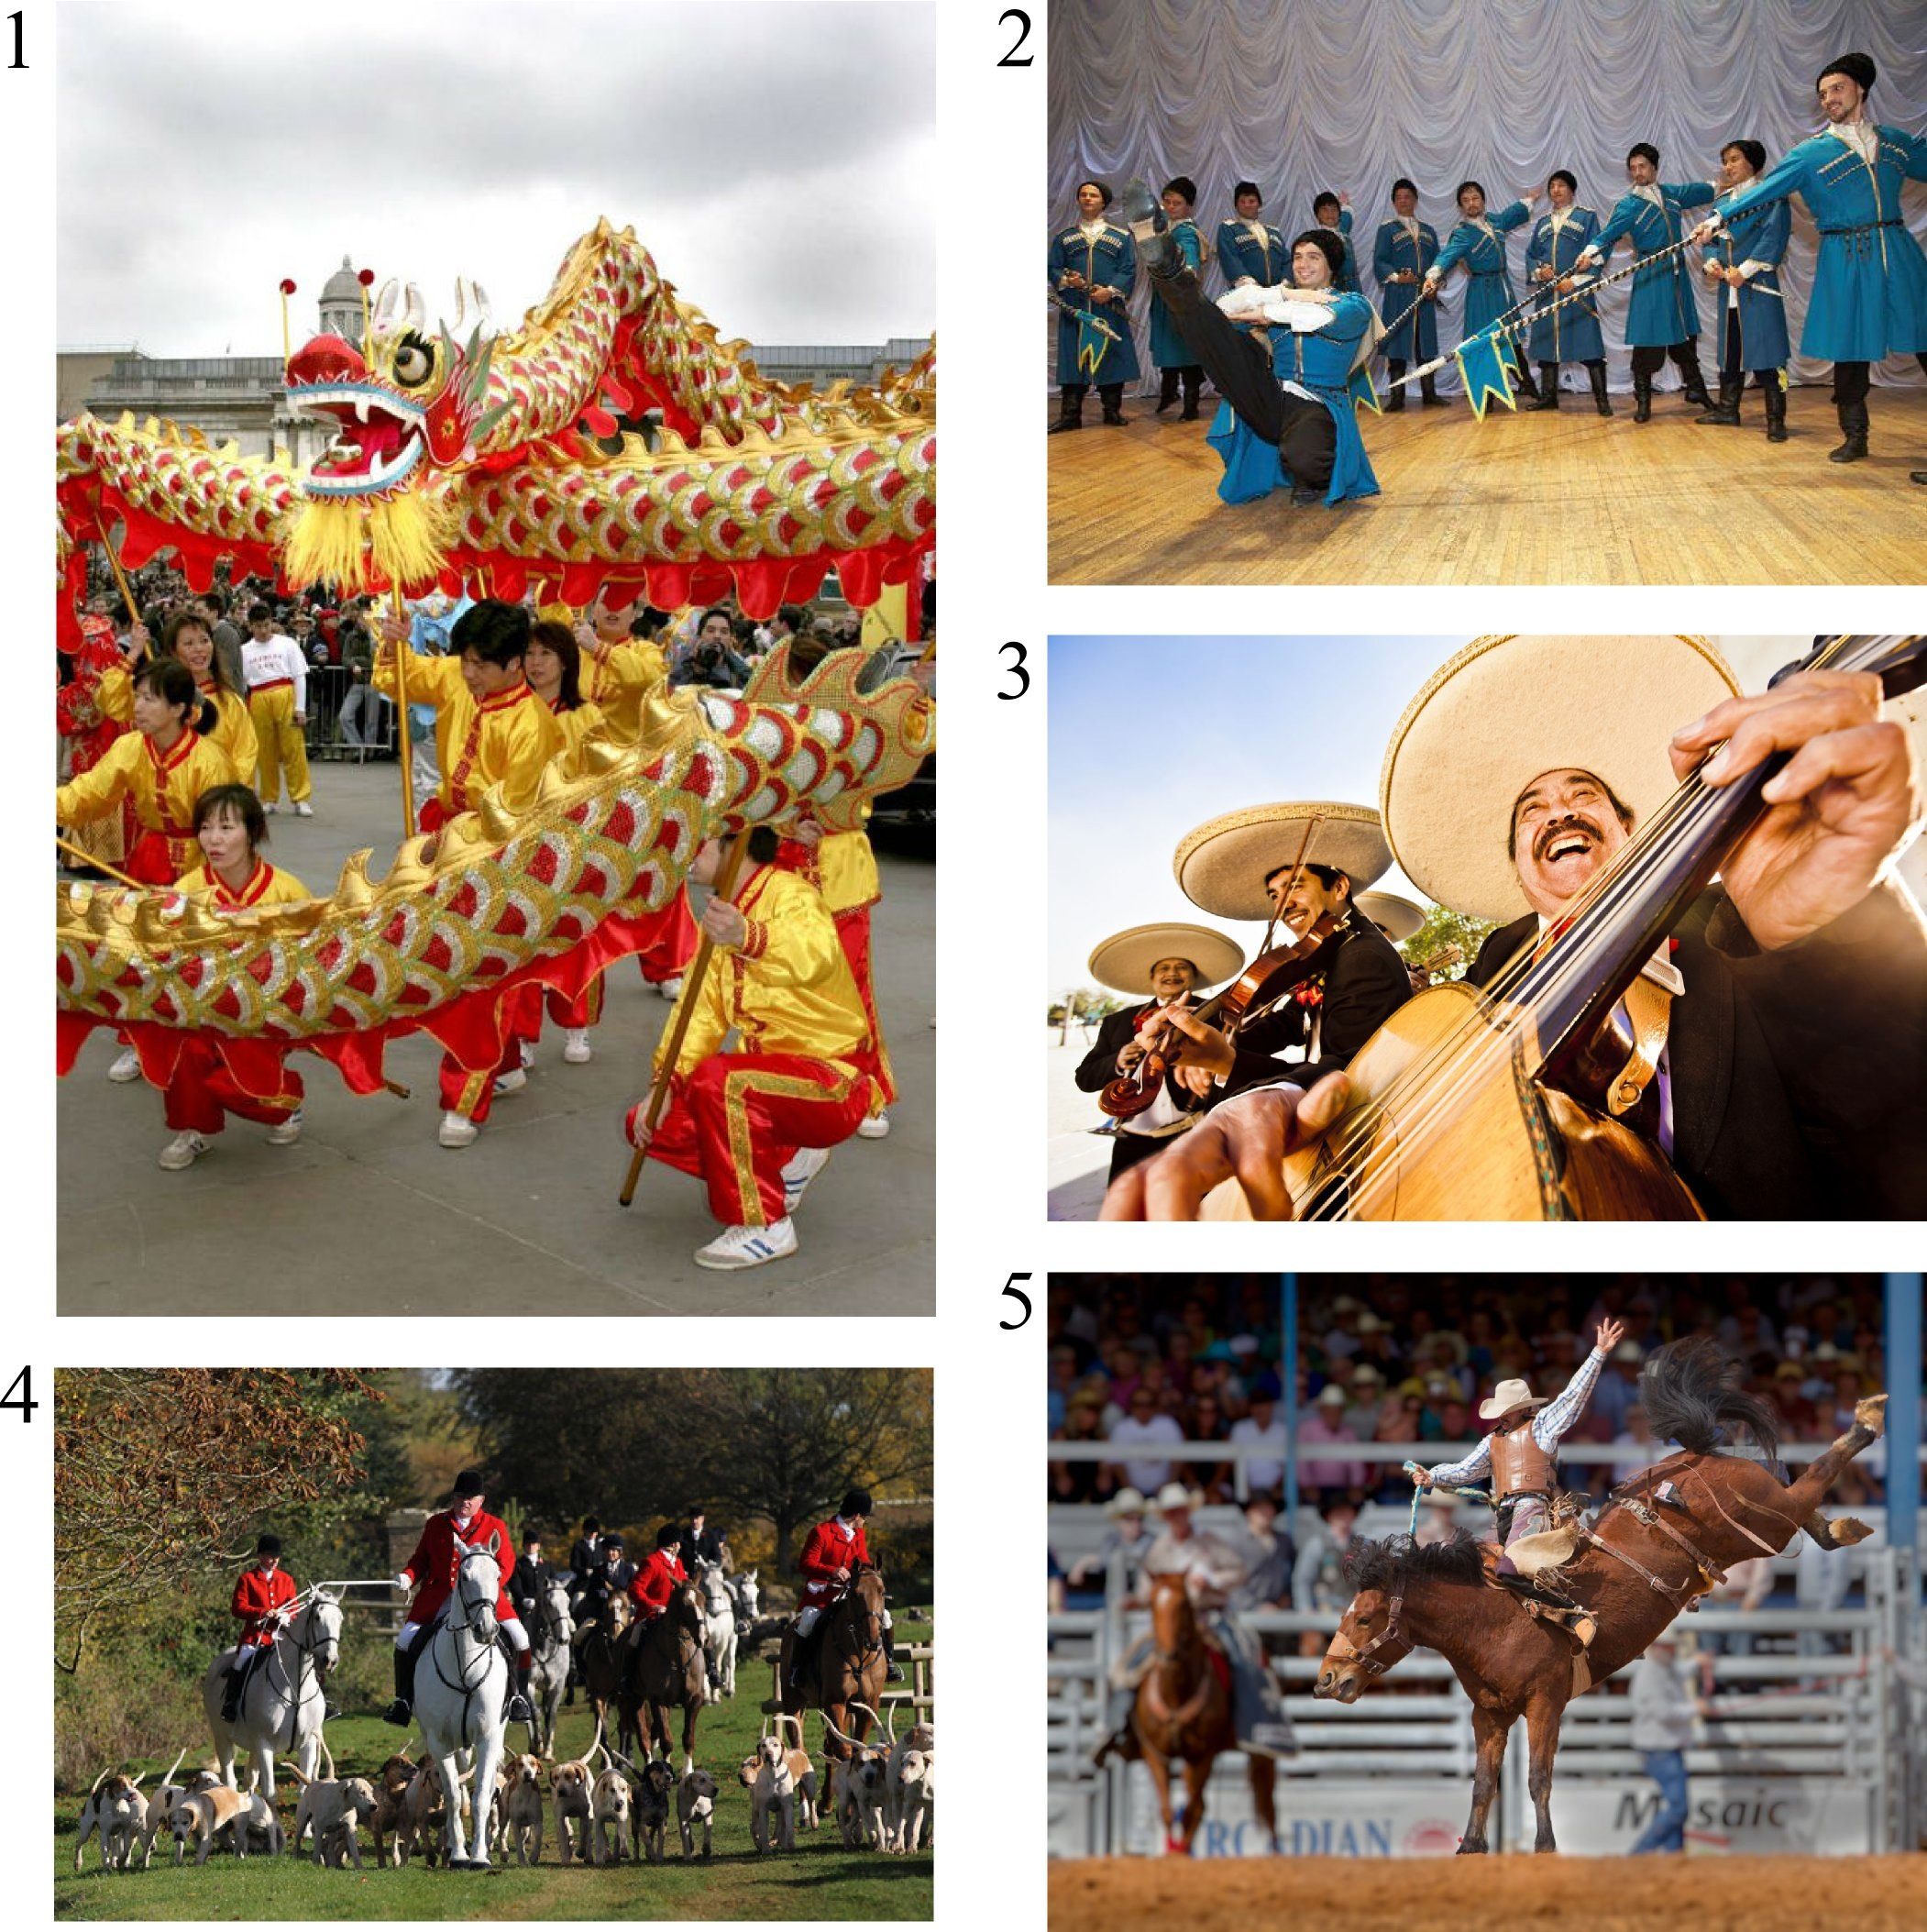
\includegraphics[scale=1.00]{../figs/taskImages/cultural.png}
	\caption{Cultural image set.  These images were chosen for their overt and
	specific cultural orientation.}
	\label{fig:cultural}
\end{figure*}

\begin{figure*}
	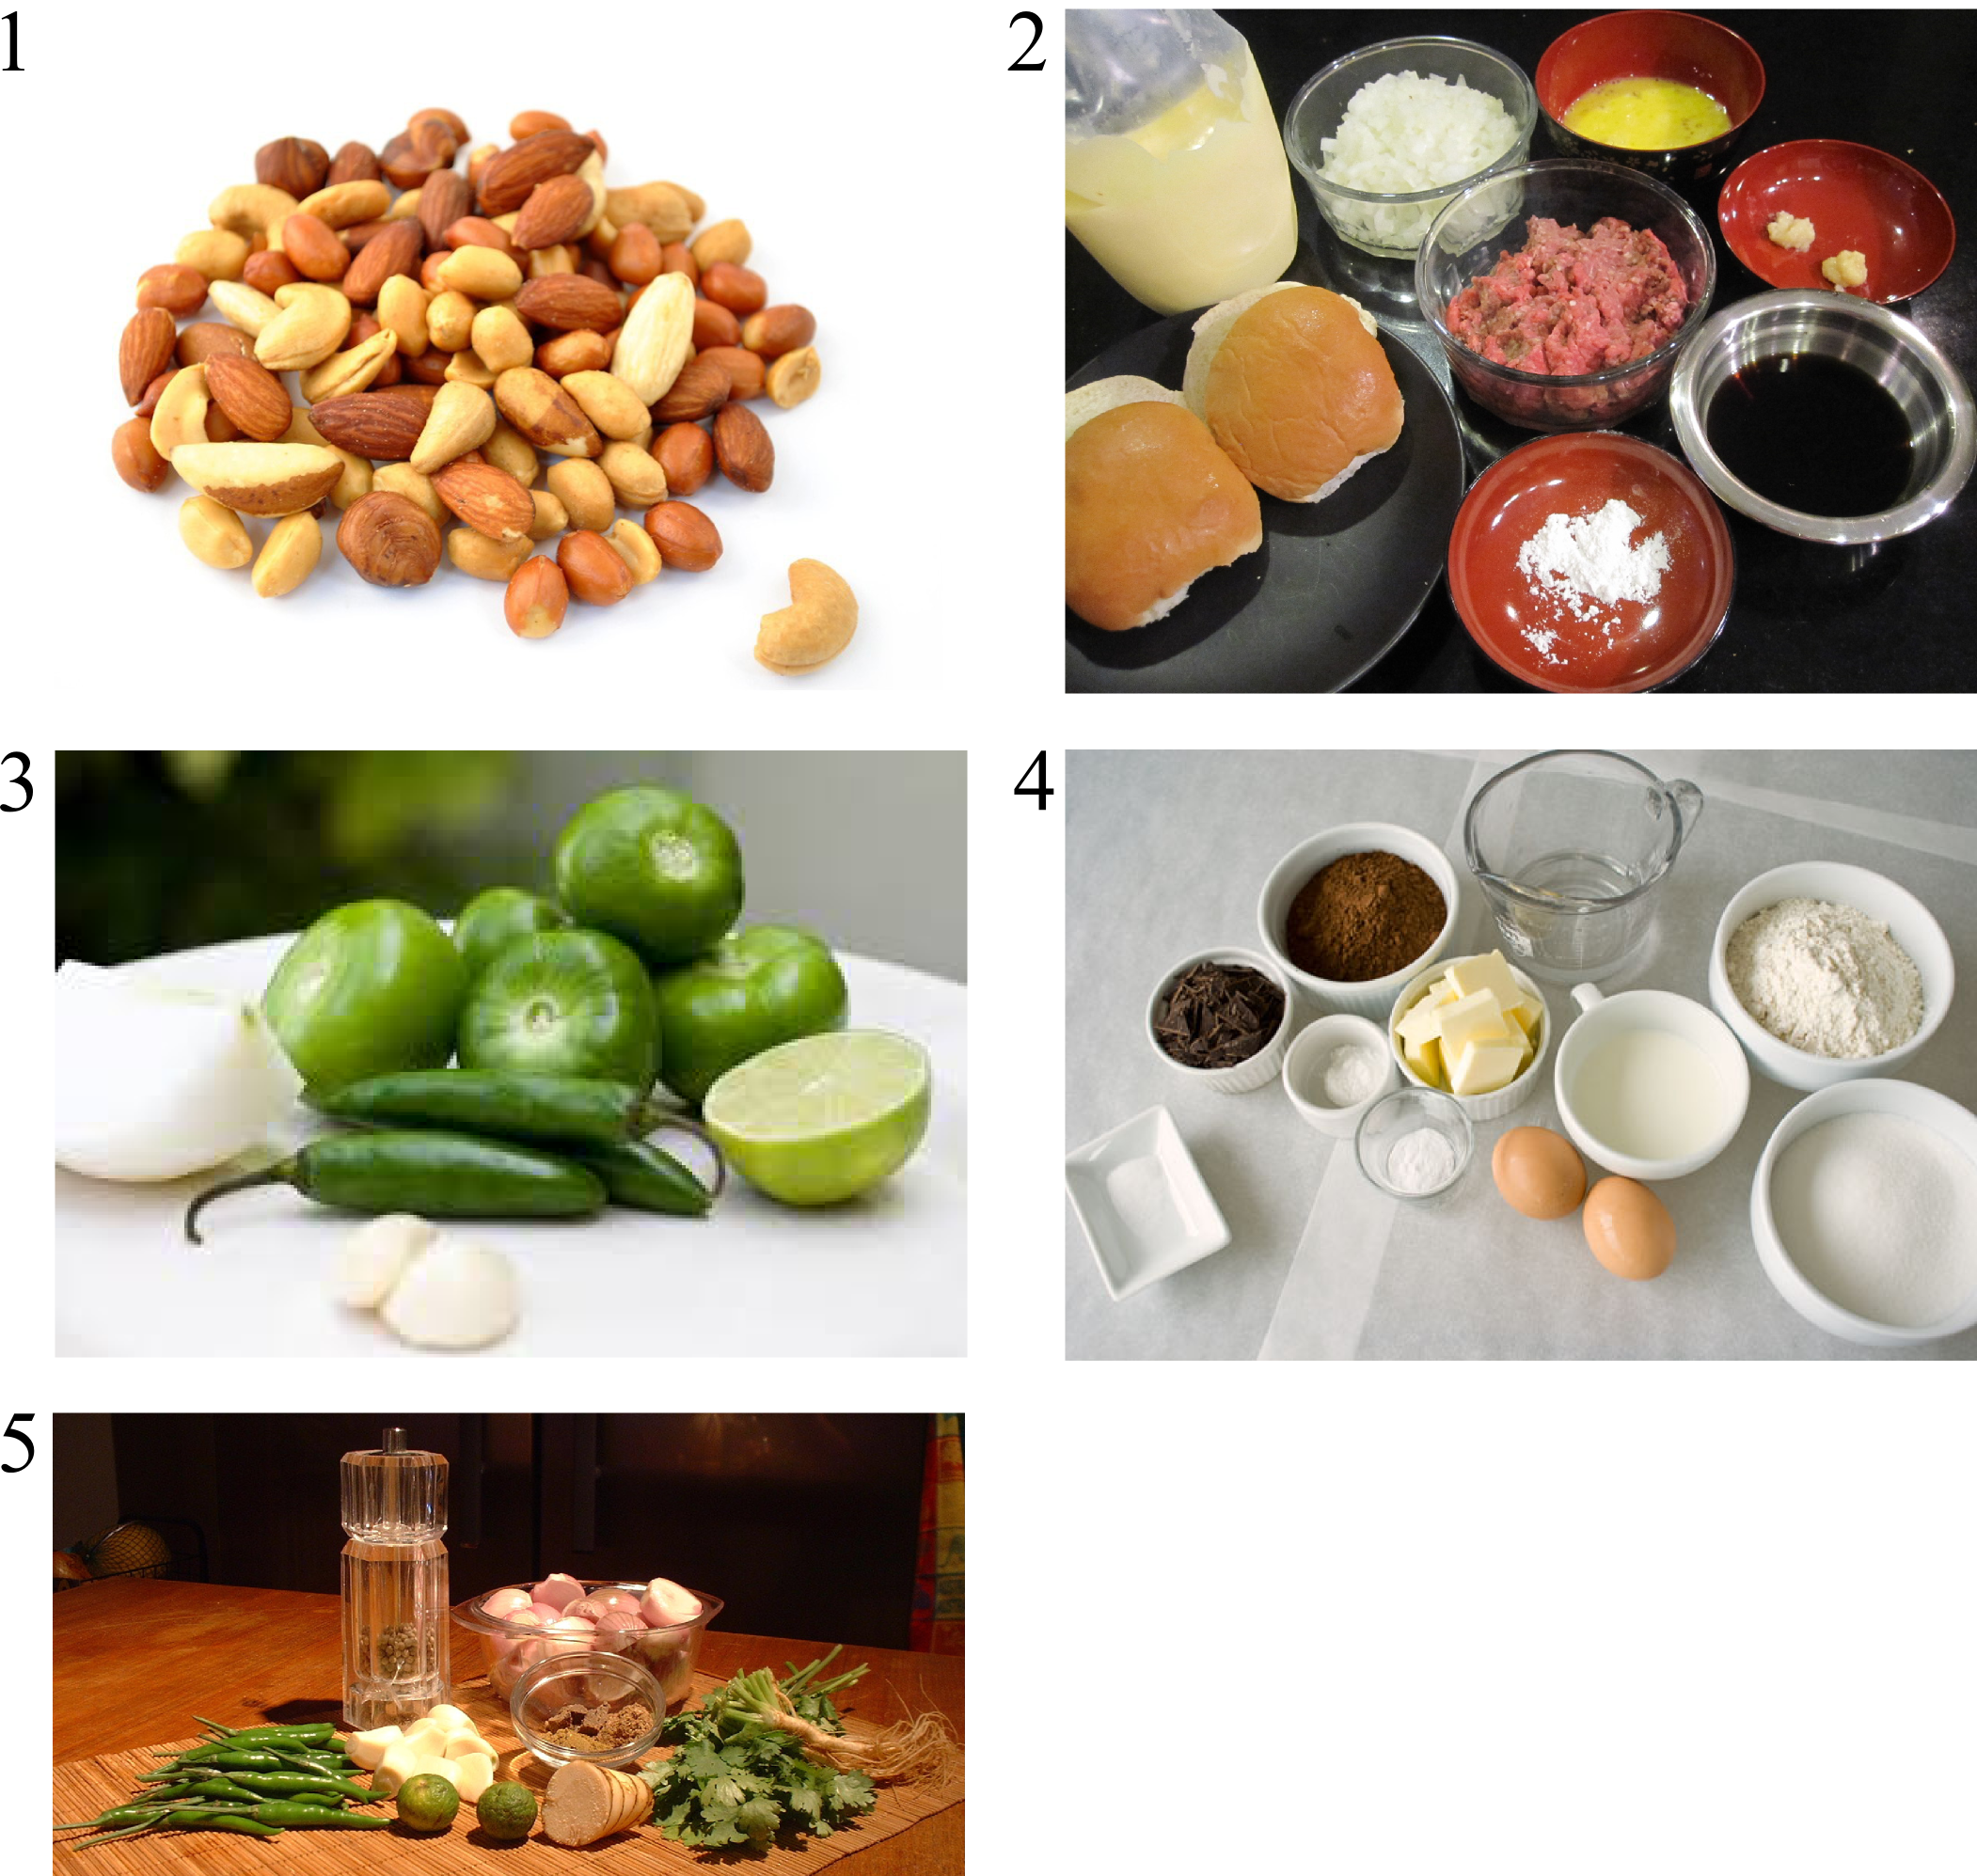
\includegraphics[scale=1.00]{../figs/taskImages/ingredients.png}
	\caption{Ingredients image set.  These images were chosen for their focus on
	food ingredients, with the intention of encouraging workers to produce labels
	of higher specificity relating to food.}
	\label{fig:ingredients}
\end{figure*}

\bibliographystyle{plain}
\bibliography{bab.bib}

\end{document}
